\documentclass{sig-alternate}
\usepackage[utf8]{inputenc}

\usepackage{comment}
\newcommand{\redcolor}[1]{\textcolor{red}{#1}}
\newcommand{\figref}[1]{Figure~\ref{#1}}
\newcommand{\secref}[1]{Section~\ref{#1}}
\newcommand{\tabref}[1]{Table~\ref{#1}}
\newcommand{\algoref}[1]{Algorithm~\ref{#1}}
\usepackage{xcolor,colortbl}

\title{NILMTK: An open source toolkit for Non-intrusive load monitoring}
\author{Nipun Batra$^1$, Jack Kelly$^2$, Oliver Parson$^3$, Haimonti Dutta$^4$, William Knottenbelt$^2$,\\ Alex Rogers$^3$,Amarjeet Singh$^1$, Mani Srivastava$^5$\\
\scriptsize$^1$Indraprastha Institute of Information Technology, Delhi, India\\
\scriptsize\{nipunb,amarjeet\}@iiitd.ac.in\\
\scriptsize$^2$ Imperial College, London\\
\scriptsize\{jack.kelly@imperial.ac.uk, wjk@doc.ic.ac.uk\}\\
\scriptsize$^3$ University of Southampton\\
\scriptsize\{op106,acr\}@ecs.soton.ac.uk\\
\scriptsize$^4$ CCLS, Columbia\\
\scriptsize\{haimonti@ccls.columbia.edu\}\\
\scriptsize$^5$ UCLA\\
\scriptsize\{mbs@ucla.edu\}\\
}


\date{December 2013}

\begin{document}

\maketitle

\section{Abstract}
Non-intrusive load monitoring, or energy disaggregation, aims to separate household energy consumption data collected from a single point of measurement into individual appliances. In recent years, the field has rapidly increased in size with the national rollouts of smart meters, and as a result many new disaggregation algorithms have been proposed. However, empirically comparing such algorithms is currently virtually impossible, as a result of the different data sets used, the lack of availability of algorithms, and the wealth of accuracy metrics which have been employed. To address this challenge, we present NILMTK; an open source toolkit designed specifically to enable the comparison of energy disaggregation algorithms in a reproducible manner. Our toolkit includes parsers to a range of existing data sets, a standard output format for disaggregation algorithms, a set of statistics for describing datasets, a reference benchmark disaggregation algorithm, and a suite of accuracy metrics. We demonstrate that our toolkit lowers the barrier to entry by simplifying the use of multiple data sets, ease of adding new disaggregation algorithms, while also encouraging direct comparisons to be made between algorithms through common output formats and accuracy metrics.

\section{Introduction}
Non-intrusive load monitoring (NILM), or energy disaggregation, aims to break down a household's aggregate electricity consumption into individual appliances~\cite{hart_1992}. The motivations for such a process are threefold. First, informing a household's occupants of how much energy each appliance consumes empowers them to take steps towards reducing their energy consumption~\cite{darby_2006}. Second, 
personalised feedback can be provided which quantifies the savings of certain appliance-specific advice, such as the financial savings when an old inefficient appliance is replaced by a new efficient appliance. Third, if the NILM system is able to determine the time of use of each appliance, a recommender system would be able to inform the household's occupants of the potential savings through deferring appliance use to a time of day when electricity is either cheaper or has a lower carbon footprint.

Such benefits have drawn significant interest in the field since its inception 25 years ago. In recent years, the combination of national smart meter meter deployments (e.g. REF UK, USA) and also decreasing hardware costs of household electricity sensors has lead to a rapid expansion of the field. Such rapid growth over the past 5 years has been evidenced by the wealth of academic papers published, international meetings held (NLM 2012, EPRI NILM 2013), startup companies founded (e.g. Bidgely, Neurio) and data sets released.

However, three core barriers are currently preventing the direct comparison of existing approaches, and as a result are limiting progress within the field. First, each contribution to date has only been evaluated on a single data set as a result of the difficulty in moving from one data set to another, and consequently it is hard to assess the generalisability of approaches. Furthermore, many papers subsample existing data sets to select specific households, appliances and time periods, making experimental results harder to reproduce. Second, newly proposed approaches are rarely benchmarked against the same algorithms, further increasing the difficulty in empirical comparisons of performance between different papers. Moreover, the lack of availability of state-of-the-art algorithms often leads to the reimplementation of such approaches. Third, each paper targets a subtly different use case for NILM and therefore evaluates the accuracy of their proposed approach using a different set of performance metrics. As a result the numerical performance calculated by such metrics cannot be compared between two papers. These three barriers have led to successive extensions to state-of-the-art algorithms being proposed, while a direct comparison between such approaches has remained impossible.

Similar barriers also have arisen in other research fields and prompted the development of toolkits specifically designed to support a given area. For example, PhysioToolkit offers access to over 50 databases of physiological data and provides software to support the processing and analysis of such data for the biomedical research community~\cite{physionet}. Similarly, CRAWDAD collects 89 data sets of wireless network data in addition to supporting software to aid the analysis of such data by the wireless network community~\cite{crawdad}. However, no such toolkit is available to the NILM community.

Against this background, we propose NILMTK; an open source toolkit designed specifically to enable the comparison of energy disaggregation algorithms. The primary aim of the toolkit is to provide a complete pipeline from data sets to accuracy metrics, therefore lowering the barrier to entry for researchers to plug in a new algorithm and compare its performance to the current state of the art. The toolkit has been released as open source software in an effort to encourage researchers to contribute data sets, benchmark algorithms and accuracy metrics as they are proposed, with the goal of enabling a greater level of collaboration within the community. In addition, the toolkit has been designed using a modular structure, therefore allowing researchers to reuse or replace individual components as required. Last, the toolkit has been written in Python with flat file input and output formats, in addition to high performance binary formats, ensuring compatibility with existing algorithms written in any language and designed for any platform.

Our contributions are summarized as follows:\begin{itemize}
\item We propose REDD+, the standard structure for energy disaggregation data sets used by NILMTK based on an extension of the format used for the REDD data set. Furthermore, we provide parsers from multiple existing data sets into our proposed REDD+ format. In addition, we propose a single output format for the disaggregated data produced by NILM algorithms.
\item We provide an implementation of a benchmark disaggregation which uses combinatorial optimization to disaggregate household energy data into individual appliances. We demonstrate the ease by which NILMTK allows comparing this algorithm across a range of existing data sets, and present results of its performance accuracy.
\item We present a suite of accuracy metrics which are able to evaluate the performance of any disaggregation algorithms which produce output compatible with NILMTK. This allows the performance of a disaggregation algorithm to be evaluated for a range of use cases.
\end{itemize}
The remainder of this paper is organized as follows. In \secref{sec:related} we provide an overview of related work from the field of NILM and also other similar fields of research. In \secref{sec:nilmtk} we present NILMTK, and give a detailed description of its components. In \secref{evaluation} we demonstrate the empirical evaluations which are enabled by NILMTK, and provide analysis of existing data sets and accuracy metrics. Finally, in \secref{sec:conclusions} we conclude the paper and propose directions for future work.

\section{Related Work}
\label{sec:related}

\redcolor{Maybe add year of release to the table also?}

\begin{table*}[]
  \centering
  \begin{tabular}{c c c c c c c c}
    \hline
    \bf Data set & \bf Institution & \bf Location & \bf Duration & \bf Number & \bf Appliance & \bf Aggregate\\
    \bf  & \bf  & \bf  & \bf  & \bf of houses & \bf sample period & \bf sample period\\
    \hline
    REDD & MIT & MA, USA & 3-19 days & 6 & 3 second & 1 second / 15kHz\\
    BLUED & CMU & PA, USA & 8 days & 1 & N/A & N/A\\
    Smart* & UMass & MA, USA & 3 months & 1 & 1 second & 1 second\\
    Sample data set & Pecan Street & TX, USA & 7 days & 10 & 1 minute & 1 minute\\
    HES & DEFRA/DECC & UK & 1 or 12 months & 251 & 2 minute & N/A\\
    AMPds & Simon Fraser U. & BC, Canada & 1 year & 1 & 1 minute & Yes\\
    iAWE & IIIT Delhi & Delhi, India & 73 days & 1 & 1 second & 1 second\\
    UKPD & Imperial College & London, UK & 3 - 14 months & 4 & 6 secs & 1 or 6 sec or 16kHz \\
    \hline
  \end{tabular}
  \caption{Table of comparison of household energy data sets.}
  \label{table:datasets}
\end{table*}

The field of non-intrusive load monitoring was founded over 20 years ago when Hart proposed the algorithmic disaggregation of household energy usage~\cite{hart_1992}. Since, many summary studies have shown the benefits of disaggregated data to both household occupants through financial savings, and also to utility providers through load shedding potential~\cite{zeifman_2011,armel_2013}. However, the majority of research had been evaluated using either lab-based data or simulated data, and as a result the performance of disaggregation algorithms in real households has remained unknown. More recently, national deployments of smart meters have prompted a renewed interest in energy disaggregation, and as a result a number of data sets collected specifically for energy disaggregation have been released. We now discuss the data sets which are currently available, which we subsequently summarise in \tabref{table:datasets}.

In 2011, the Reference Energy Disaggregation Dataset (REDD)~\cite{redd} was the first data set to be released which was collected specifically to aid NILM research. The data set contains both aggregate and sub-metered power data from 6 homes, and has since become the most popular data set for evaluating energy disaggregation algorithms. The following year, the Building-Level fUlly-labeled dataset for Electricity Disaggregation (BLUED) was released containing data from a single household. However, the data set does not include sub-metered power data, and instead events were recorded each time an appliance changed state (e.g.\ turned on). As a result, it is only possible to evaluate how well appliance activity can be inferred, rather than the disaggregation of appliance energy consumption. More recently, the SMART*~\cite{smart} data set was released, which contains household aggregate power data from 3 homes, while sub-metered appliance power data was only collected from a single household.

In 2013 the Pecan Street Sample data set was released~\cite{pecan}, which contains both aggregate data and sub-metered data from 10 households. Later, the Household Energy Study data set was released, which contains data from 250 households although only sub-metered appliance data was collected. Also that year, the Almanac of Minutely Power dataset (AMPds)~\cite{ampds} was released which contains both aggregate and sub-metered data from a single household. Subsequently, the Indian data for Ambient Water and Electricity Sensing (iAWE)~\cite{iawe} was released, which contains both aggregate and sub-metered electricity data from a single home. Most recently, the UK Power Data (UKPD)~\cite{?} was proposed which contains data from four households using both aggregate meters and individual appliance sub-meters. Unfortunately, subtle differences in the aims of each data set have lead to completely different data formats being used, and as a result a significant engineering barrier exists when moving from one data set to another. This has resulted in publications using only a single data set to evaluate a given approach, and consequently the generality of results are rarely investigated. Having described the data sets that are currently available, we now discuss recent publications which have used such data sets for the evaluation of disaggregation algorithms.

The REDD data set has been used to compare the performance of many disaggregation algorithms since its publication in 2011. The data set was proposed along with a performance result of a benchmark disaggregation algorithm using low frequency data across 5 of the 6 households~\cite{redd}. Kolter and Jaakkola later proposed an extension to the benchmark algorithm~\cite{kolter_2012}, however the extension was only evaluated using high frequency data from a single home from the data set, and therefore the performance results are not directly comparable. Later, Zeifman~\cite{zeifman_2012} and Johnson and Willsky~\cite{johnson_2013} evaluated various approaches using the same data set, although both selected a different subset of appliances and calculated an artificial household aggregate from these appliances, therefore simplifying the disaggregation problem and preventing a numerical comparison with other publications. Subsequently, Parson et al.~\cite{parson_2012} and Rahayu et al.~\cite{rahayu_2012} both proposed new approaches, although each were evaluated using a different set of 4 houses from the REDD data set, again preventing a numerical comparison between publications. Last, Batra et al.~\cite{batra_2013} evaluated their approach on the REDD data set using a different household to Kolter and Jaakkola, again preventing a direct performance comparison of numerical results. As a result, it has not been possible to deduce whether one approach is preferable to another from the literature.

In addition to REDD, other data sets have also been used to evaluate the performance of NILM algorithms. For example, BLUED was introduced along with a benchmark algorithm~\cite{blued}, but has since only been used by one other publication~\cite{anderson_2012}. Similarly, AMPds and iAWE have only been used to evaluate disaggregation algorithms proposed by the data set authors~\cite{ampds,iawe}. Clearly, the variety of different formats is preventing the uptake of new data sets, and also preventing algorithms from being tested across multiple data sets. Having discussed the open data sets used by recent publications, we now describe the benchmarks against which newly proposed disaggregation algorithms have been compared.

It is essential to compare newly proposed disaggregation algorithms to the state of the art in order to assess the increase in an algorithm's performance. However, the lack of availability of state-of-the-art disaggregation algorithms has led to authors often comparing against more basic benchmark algorithms. This problem is further compounded since there is no single consensus on which benchmark to use, and as a result most publications use a different benchmark algorithm. For example, Kolter and Jaakkola compared their approach to a set of decoupled HMMs~\cite{kolter_2012}, Parson et al.\ and Batra et al.\ both evaluated their approaches against variants of their own approaches~\cite{parson_2012,batra_2013}, Zeifman compared their approach to a Bayesian classifier, while Rahayu et al. and Johnson and Willsky both compared against a FHMM~\cite{rahayu_2012,johnson_2013}. Clearly, further publications would benefit from openly available common benchmark algorithms against which newly proposed algorithms could be easily compared. Having discussed benchmark approaches, we now describe the various metrics which have been used to compare disaggregation algorithms.

The range of different application areas of energy disaggregation has prompted a number of evaluation metrics to be proposed. For example, four disaggregation metrics labelled \emph{energy correctly assigned} have recently been used to evaluate the performance of disaggregation algorithms using the REDD data set. First, Kolter and Johnson~\cite{redd} proposed the use of an accuracy metric which captures the error in assigned energy normalised by the actual energy consumption in each time slice averaged over all appliances, which was also later used by Rahayu et al.~\cite{rahayu_2012} and Johnson and Willsky~\cite{johnson_2013}. However, large errors in the assigned energy in some time slices will result in a negative accuracy, making this an ill-posed metric. Second, Kolter and Jaakkola~\cite{kolter_2012} proposed an equivalent metric, although the error is presented individually for each appliance rather than an average across all appliances. Third, Parson et al.~\cite{parson_2012} proposed a similar metric, although the metric captures the error in assigned energy consumed over the complete duration of the data set rather than per time slice. However, this metric allows overestimates and underestimates in the assigned energy in different time slices to cancel out, and therefore does not represent all disaggregation errors. Fourth, Batra et al.~\cite{batra_2013} proposed a subtly different metric to Kolter and Johnson~\cite{redd}, in which error is reported instead of accuracy, and also energy assigned to an incorrect appliance is double counted. Each of the differences between these four metrics prevents a numerical comparison between publications, and motivates the use of common metrics.

\section{NILMTK}
\label{sec:nilmtk}
NILMTK aims to address the following three design goals:
\begin{itemize}
\item \textbf{Analysis}: The toolkit should facilitate easy analysis of NILM datasets and expose the entire pipeline from
data importing through disaggregation to metrics. 
\item \textbf{Ease of adding new algorithms}: The toolkit should provide consistent interfaces for new disaggregation algorithms.
\item \textbf{Ease of deploying}: The toolkit should be built in such a way that the learnt model is easily deployable and can interface with online as well as offline data.
\end{itemize}
Based on these three design goals, we chose to implement NILMTK in Python. Python is increasingly becoming popular for data science, machine learning and open science. Python allows easy deployment in diverse environments including academic settings. The availability of a vast set of libraries ranging from statistical analysis (Pandas), machine learning (Scikit-learn), web frameworks (Django), etc, make it a suitable choice for our toolkit. Further, the availability of Python on low cost platforms such as Raspberry Pi allows ease of deployment.

Our API design is heavily based on scikit-learn~\cite{scikit, scikit_api}, which is a well known machine learning framework in the Python community. Scikit-learn is designed for general purpose machine learning tasks and has set high code standards. However, as pointed earlier in \secref{sec:related}, the domain specifics of NILM demand a specialized framework. We present below the NILMTK pipeline from importing dataset to evaluation over NILM specific metrics.

\subsection{Mathematical conventions}
In this section we briefly introduce the mathematical conventions we use throughout the rest of this paper. The power draw by $i^{th}$ appliance at time $t$ is given by . Most of the NILM algorithms model appliances to have multiple states such as off, on, intermediate, etc. The state of $i^{th}$ appliance at time $t$ is given by ..where .. belongs to ${1..k}$

\subsection{NILMTK pipeline}
In this section we describe the implementation and design of NILMTK pipeline. 
\subsubsection{Dataset Importers} As pointed in \secref{sec:related}, a number of datasets have been released in the recent past. The differences between these datasets has been a cause of low adoption and thus, there are limitations on the ease of NILM comparison. Motivated by this, we decided to import all the existing datasets into a common format based on the REDD format, which we call REDD+. We chose to keep the format relatively close to REDD, so that tools developed for REDD would be able to use our format with little or not modification. 

We provide both CSV flat files based format and a much more efficient Hierarchical Data Format (HDF5) binary file format. At the time of writing, we have written REDD+ converters for the following datasets: REDD, PECAN, HES, iAWE, AMPds, UKPD. In addition to storing electricity data, REDD+ format allows storing relevant metadata and other sensor modalities such as gas, water, temperature, etc. It has been shown in the past that additional sensor and metadata information may help enhance NILM prediction.\redcolor{Add citations}. A detailed account of the REDD+ format has been provided in the appendix. 

Another important feature of our format is naming standardization. Appliances are referred by vairous names in different datasets. \redcolor{Jack: Wanna write this bit? Give some examples and explain a few advantages we get by naming standardization. Explain the source of these and how these relate to wiki. 
}

\subsubsection{Preprocessing} The datasets described above have been collected with a multitude of hardware, with different aims and under different setting. As shown in \tabref{tab:dataset} the sampling frequency of appliance monitors varies from 1 second to 2 minutes across the datasets.  We thus created filters for downsampling datasets via different filters such as mean, median etc. Further, these datasets have been collected in different countries, where the voltage fluctuations are varied. Batra et. al showed voltage fluctuations from 180-250 V in their iAWE dataset~\cite{iawe} collected in India. The corresponding numbers in SMART* are 118-123 V. Hart et. al~\cite{hart_1992} showed the need to factor these voltage fluctuations as they significantly impact power draw. Thus, we also add a voltage normalization preprocessor function which is defined as follows. 
$$Power_{normalized} = (\frac{Voltage_{observed}}{Voltage_{nominal}})^2.Power_{observed}$$
Figure x shows the power draw of an air conditioner, before and after voltage normalization. As we explain in the algorithms section below, some algorithms for NILM are exponential in the number of appliances. Thus, when the number of appliances are considered for NILM, the models do not fit into memory and distributed models need to be considered. This necessitates the need to filter out top-k appliances by their contribution which can be in terms of energy or power.  We also created preprocessing functions for fixing some common issues with domestic power data. In section evaluation, we compare the NILM results when k in top-k were varied. A summary of preprocessing functions is provided in table.

\subsubsection{Statistics}

\redcolor{Jack will write this ASAP}

\subsubsection{Cross Validation} 

\subsubsection{Training and Disaggregation} In the current release of NILMTK, we provide two benchmark NILM algorithms: 1)Combinatorial optimization(CO); and 2)Factorial Hidden Markov Model(FHMM). CO was proposed by Hart in his seminal work, while techniques based on Hidden Markov Models(HMMs) such as FHMM constitute the state of the art. It should be highlighted that the intended purpose of these algorithms is only to serve as benchmarks. We do not claim these to give the best results. We would encourage the community to get involved and submit their algorithms to NILMTK. Now we briefly describe these two algorithms.

\noindent \textbf{Combinatorial Optimization:} CO tries to find the \textit{optimal} combination of appliances in different states, the sum of which matches most closely to the observed power at aggregate level.  Its mathematical formulation is given as follows. CO assumes time samples to be independent and identically distributed (iid). CO resembles the subset sum problem and thus is NP-hard. The complexity of disaggregation for each time slice is $O(K^N)$, where N is the number of appliances. Since the space and time complexity of CO is exponential in terms of number of appliances, the approach does not scale well.

\noindent \textbf{Factorial Hidden Markov Model:} The power draw of each appliance can be considered to be the observation of a Gaussian HMM. The hidden component of these HMMs are the states of the appliances. However, the task at hand involves jointly decoding the power draw of n appliances and hence a Factorial HMM~\cite{fhmm} is well suited. A Factorial HMM can be represented by its equivalent HMM. The complexity of disaggregation for each time slice is $O(K^2N)$. FHMMs scale even more poorly than CO. From an implementation perspective, even storing the model for 12 appliances with 2 states each will need X GB of RAM. Hence, we propose to validate FHMMs on top-k loads.



\subsubsection{Model import and export} Recently, a lot of interest has arisen in real life systems doing NILM. Startups such as Neurio, PlotWatt, Bidgely, etc. have recently surfaced and provide disaggregated consumption feedback to end consumers. A major barrier which existed previously was that the academic algorithms were produced merely for static analysis. Motivated by reducing the barrier to deployable algorithms, we developed Model module in NILMTK. It is the responsibility of the model developer to create export and import functions to interface with a JSON file. We provide the importers and exporters for FHMM and CO. Further, in the use case section, we show how if the rated power is known, we can avoid learning on sub-metered data. At the time of deployment, this learnt JSON model can be easily imported and disaggregation performed.

\subsubsection{Metrics}


We summarize the NILMTK pipeline with an illustrative code snippet.
\begin{verbatim}
# Add a minimal example to illustrate all aspects of the approach
dataset = DataSet()
t1 = time.time()
dataset.load_hdf5(EXPORT_PATH)
\end{verbatim}


\section{Evaluation}
\label{evaluation}
\subsection{The curious case of voltage normalization}
\subsection{Effect of sampling rate}
\begin{figure*}
\centering 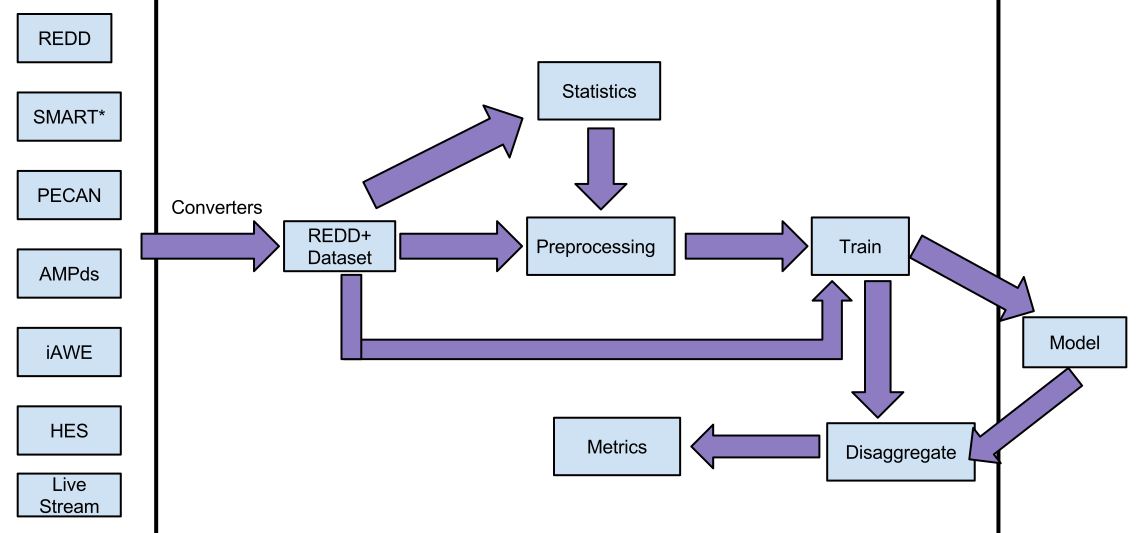
\includegraphics[scale=0.4]{figures/pipeline.jpg}
\caption{NILMTK pipeline}
\label{fig:pipeline}
\end{figure*}


\begin{tabular}{|c|c|c|c|c|c|c|c|}
\hline
Appliance(n) & Main & \multicolumn{6}{|c|}{States Power (W)}\\
\hline
&&\multicolumn{3}{|c|}{Pre calibration}&\multicolumn{3}{|c|}{Post calibration}\\
\hline
             &  &$\mu^n_1$&$\mu^n_2$&$\mu^n_3$&$\mu^n_1$&$\mu^n_2$&$\mu^n_3$\\[0.1cm]
\hline
Refrigerator & 2& 7&162&423 & 7&214&423\\
%\footnote{There were not enough instances of refrigerator in state 3 to calibrate it}\\
Microwave &2& 9&822&1740& 9&822&1740\\
Lighting & 2& 9&96&156&9&113&156\\
Dishwasher & 1& 0&260& 1195 & 0&260& 1195\\
Stove& 1 & 0&373&-& 0&373&-\\
Kitchen & 1& 5&727&-&5&727&-\\
Kitchen 2&1 & 1&204&1036&1&204&1036 \\
%
%
\hline
%
\end{tabular}

\section{Discussion}

\section{Conclusions and future work}
\label{sec:conclusions}

\section{Acknowledgments}
The authors would like to thank TCS Research and Development for supporting the first author through PhD fellowship. We would also like to thank Department of Electronic and Information Technology (DEITy), Government of India for funding the project (Grant Number DeitY/R\&D/ITEA/4(2)/2012)
\bibliographystyle{abbrv}
\bibliography{reference}

\end{document}

